\section{Background}
\label{background}

The power grid is composed of power generation, transmission, distribution and loads. Traditionally, power is generated in mass quantities from hydro, coal, nuclear, and gas sources. The power is then transmitted at high voltages to distribution systems where the power is distributed to residential and commercial consumers. As the power grid is moving towards a smarter grid, the efficient energy management is increasingly dependent on the underlying communication network supporting reliable information transfer among the various entities in the grid.

With distributed power generation---such as solar and wind energy---and more storage technology, there is a need for understanding the state of the power network in real time. A challenge with the integration of such generation, is the uncertainty and intermittency of the availability of power generation.
In order to combat this challenge, there needs to be an infrastructure that allows for the monitoring and control of the system state. To do this effectively, requires a reliable and resilient communication network.

Researchers have developed systems to co-simulate the power and network components of the smart grid \cite{DSSco-sim, DSS-RT-HIL, RT-SmartGrid, GECO, EPOCHS, FNCS, FNCS-algos}. \cite{Mets2014} surveys the existing technologies and motivations for co-simulation.

In \cite{DSS-RT-HIL}, a system is proposed using OpenDSS to allow for sending real-time signals to hardware integrating with simulation.
Real time simulators are used for hardware-in-the-loop simulations, allowing for simulation-emulation closer to the real system \cite{RT-SmartGrid}. This gives high fidelity, but requires power equipment and often specific simulator hardware.
While real-time simulators exist, they are costly and often require specific hardware to operate, our challenge is to design a hardware-in-the-loop testbed that can use standard electric power simulators that run slower than real-time while maintaining temporal fidelity.

In \cite{GECO}, the authors create a co-simulation between PSLF and ns-2.
They use a global event driven mechanism for sending synchronization messages between the two simulators.
In simulation, events are sorted by time stamps, typically in a priority queue and are executed as fast as possible without regard to the wall clock.

EPOCHS \cite{EPOCHS} uses commercial power simulators to co-simulate network and power systems through the use of agents.
%While agents are not new to simulation,
This platform uses agents to effectively co-simulate power and communication elements.
The authors define agents as having the properties of autonomy and interaction.
That they exhibit properties of mobility, intelligence, adaptivity and communication.
In our design, our models run real processes on real hardware but can influence and extract values from the power simulator.
This allows for us to make use of agents to as entities that exist in both systems.

FNCS \cite{FNCS} is a federated approach for co-simulation of power and electrical simulators by combining multiple power simulators, both distribution and transmission and use ns-3 as a communication simulator.
In \cite{FNCS-algos}, the same authors improve the synchronization between systems.
The difference is that our approach is focused on running real network processes which has different synchronization challenges due to the inherent difference between the execution mechanisms in simulation and real-time processes.

There are two main features that set our design apart from the existing tools.
The first is that we are using real hardware for networking components rather than a simulator.
The second is that our testbed's design works without real-time simulators making our apporach general and low-cost.



\if 0
\section{motivation}
\label{motivation}
\fi


\section{Project Goals}

While simulation systems offer a convinient and low cost method of perfoming evaluation on models of systems it lacks the fidelity that real systems contain.

This project aims to achieve the following:
\begin{itemize}
  \item create a distributed system composed of embedded linux devices including general purpose and router devices.
  \item provide synchronization solution for real-time processes to synchronize with a discrete time step solution electric power simulator.
  \item establish a distributed emulation system
\end{itemize}


The challenges in the creation of such testbed stem for the synchronization issues between nodes in the distributed system, the processes running on the nodes, and the simulator. Specifically we will implement the following in a testbed consisting of 5 nodes, a embedded router, 2 Banana Pi devices, and 2 Raspberry Pi linux devices:

\begin{itemize}
\item Creating a kernel module that provides a user-space utility for sending hardware interrupts between the devices in the system.
The distributed synchronization between the devices is decentralized with the kernel module.
  \item Time synchronization strategy with the simulation server.
  \item Modify the scheduler to control process execution.
\end{itemize}

\begin{figure}
  \centering
  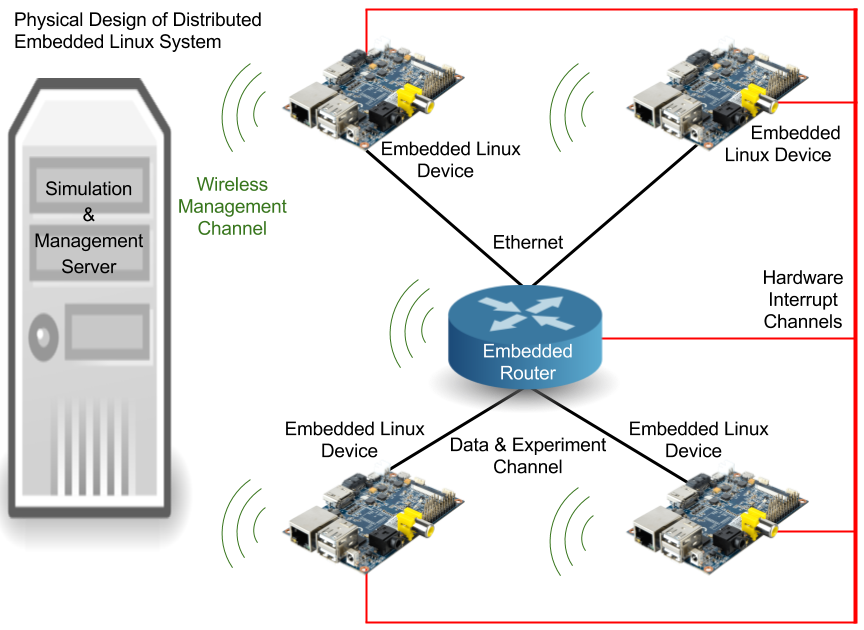
\includegraphics[scale=0.28]{Updated_architecture_emb-vt.png}
  \caption{
    Architecture of distributed system composed of 3 communication channels: Ethernet, wireless management, and direct hardware connection with general purpose and router linux hardware.
    }
\end{figure}


\section{Design}
The design of the testbed includes 2 main components: the simulation and management server, and the distributed embedded communication network system.

\subsection{Simulation and Management Server}

\subsection{Distributed Linux System}

\subsection{Synchronization Challenges}
While it is possible to run electric power simulation in real-time \cite{rt-sim}, such simulators often require specialized hardware and proprietary closed software. Thus real-time simulation is infeasible for low-cost hybrid testbeds. Additionally, the real-time nature of power simulation can not account for the exchange of messeges with the network system for passing messages.

Therefore due to the nature of the electric power simulator, it must run slower than real time.
This is inharently different from the way that commmunication systems and communication emulation systems execute.

A simulation system can be thought of a queue of events with associated time stamps.
Each event may change the state of the system, and create new events.
When a simulator progresses in time, it simply processes the next event and moves the simulation clock to the time of the event. In the case of time-step simulation, the maximum progrression of time is the size of the time-step.

On the other hand, emulation and real systems' clocks progress with the real wall clock time. This difference in the systems can lead to temporal error. To remedy this problem we utilize the virtual time kernel \cite{Yan:VTS:pads15},\cite{Yan:VTM:sosr15} based off \cite{Lamps:TK:pads14} and expand it to work on Arm32 processor family. Additionally one of the major design differences is the distributed nature of our communication network.



\begin{figure}
  \centering
  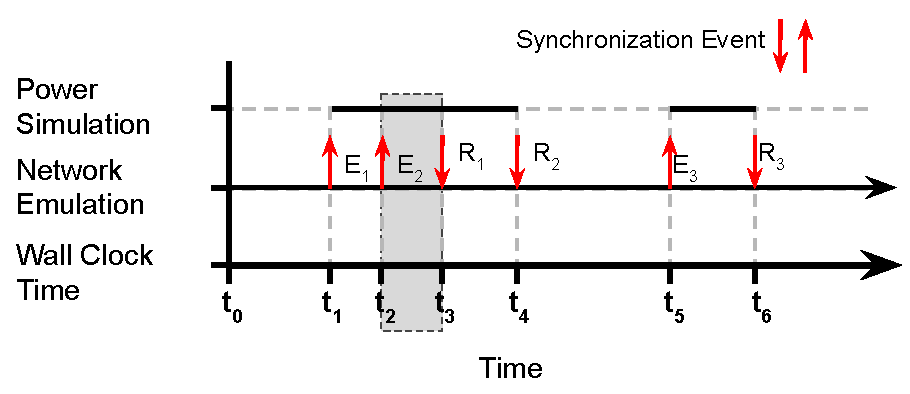
\includegraphics[scale=0.5]{no-pause-error.pdf}
  \label{sim-err}

  \caption{
    The execution of the system is shown with respect
    to the wall clock. The network (emulation) runs concurrently
    with the power simulation, and is not paused which allows
    for synchronization errors to occur, when requests arrive be-
    fore the responses are sent, i.e., $R_1$ occurs after $E_2$. The
  shaded box highlights the location of the error.}
\end{figure}

In Figure \ref{sim-err}, there are three cross-system events ($E_i$), each
with a response ($R_i$). $E_1$ occurs before $E_2$, however, $E_2$ may
require information from $R_1$. Since the response occurs after
the second event, the global causality is violated, and thus
reduces experiment fidelity. An example of $_1$ is a request
to retrieve power flow values while $E_2$ sets the value of a
discharging battery based on the value returned previously.
Since the reply $R_1$ occurs after $E_2$ this can introduce an
error. Furthermore, such errors can be accumulated if the
simulation keeps out of synchronization with the emulation.

\begin{figure}
  \centering
  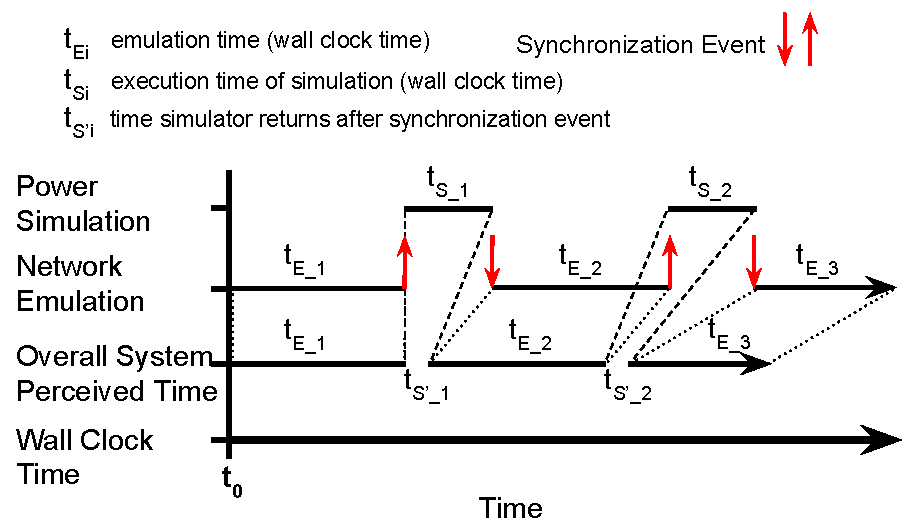
\includegraphics[scale=0.5]{wall_clock.pdf}
  \label{sim-err}

  \caption{
    The execution of the system is shown with respect
    to its own perceived time, i.e., the sum of the emulation
    execution time (can be dilated or not dilated) and the virtual
    time elapsed in simulation. The network emulation is paused
    to allow for the simulation to catch up to the emulation—
    this also ensures synchronization errors in the early example
    do not occur.
  }
\end{figure}


\section{Implemenation}

\

\section{Evaluation}

\section{Conclusion and Future Work}
We present an distributed embedded linux device testbed, a testing platform that combines an
electrical power system simulator and real communication network and distributed emulator platform. This tesbed can be used to model and simulate power flows, communication networks, and smart grid control application, and to evaluate the effect of network applications on the smart grid. Our future work includes
exploring means to extract emulation lookahead to improve
the performance of this hybrid system, as well as evaluating the scalabilityof the testbed for large-scale experiments. We also plan to investigate several novel SDN
applications for microgrid security and resilience, such as context-aware intrusion detection with PMU networks. Finally to improve the performance of the virtual time system we plan to explore real-time linux operating systems including direct control over the linux scheduler.
